\section{Nota teórica}
En esta sección del laboratorio, se exponen los principales componentes que usarán para el proyecto a realizar: un voltímetro.
\subsection*{Arduino UNO}
Se usará la placa de Arduino UNO que posee el microcontrolador ATMega382P.

\subsubsection*{Características generales}
Sus detalles se describen a continuación:
\begin{itemize}
\item Es un MCU de 8 bits.
\item Posee arquitectura RISC/Harvard.
\item 4/8/16/64 kb memoria flash.
\item 512b/1/2kb de memoria SRAM.
\item 1/2kb de EEPROM.
\item 23 GPIOS.
\item Timer/Counters de 8 y 16 bits.
\item Posee interrupciones.
\item 8 canaels PWM y comparador analógico.
\item 6 canales 10-bit ADC.
\item Posee protocolo SPI y USART (Universal Synchronous/Asynchronous Receiver/Transmitter) I2C.
\end{itemize}
\subsubsection*{Diagrama de bloques y pines}
El diagrama de bloques de este MCU se muestra en la figura \ref{fig1}.

\begin{figure}[H]
\centering
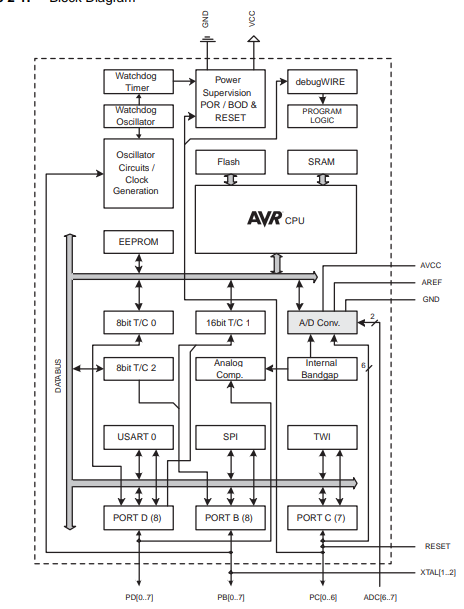
\includegraphics[width=.8\linewidth]{Imagenes/1.png}
 \caption{Diagrama de bloques de ATMega328P. Tomado de \cite{web}.}
 \label{fig1}
\end{figure}

\begin{figure}[H]
\centering
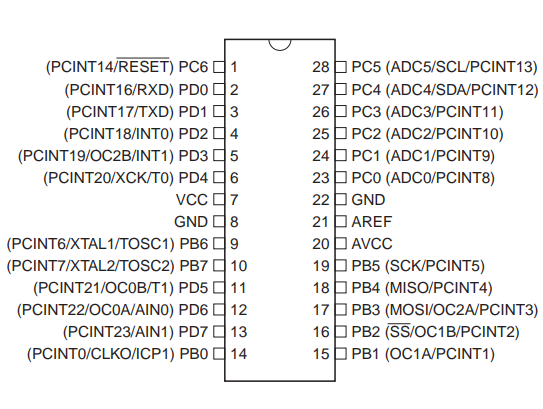
\includegraphics[width=.8\linewidth]{Imagenes/2.png}
 \caption{Diagrama de pines de ATMega328P. Tomado de \cite{web}.}
 \label{fig2}
\end{figure}
\subsubsection*{Características eléctricas}
La siguiente lista describe estos detalles.
\begin{itemize}
\item Voltaje: 1.8-\SI{5.5}{\volt}.
\item Velocidad: 0-\SI{4}{\mega\Hz},  1.8-\SI{5.5}{\volt}. 0-\SI{10}{\mega\Hz},  2.7-\SI{5.5}{\volt}. 0-\SI{20}{\mega\Hz},  4.5-\SI{5.5}{\volt}
\item Modo activo: \SI{0.3}{\mA}
\item Temperatura de funcionamiento: $-55^\circ$ a +$125^\circ$.
\item Temperatura de almacenamiento: $-65^\circ$ a +$125^\circ$.
\item Temperatura pin RESET y GND: -\SI{0.5}{\volt} a \SI{13}{\volt}.
\item Temperatura en los demás pines: -\SI{0.5}{\volt} a VCC\SI{0.5}{\volt}.
\item Corriente por pin I/O: \SI{40}{\mA}.
% AQUI SE DEBE MENCIONAR LOS PINES QUE SE USARON EN EL ARDUINO.

\end{itemize}

\subsection*{Periféricos utilizados}
Algunos periféricos usados del microcontrolador así como la pantalla PCD8544 fueron los siguientes:
\begin{itemize}
\item \textbf{pinMode:} esto se usó para cual pin era una entrada o salida, y esto ayuda para que el microcontrolador entienda todas las acciones que se desea realizar.
\item \textbf{digitalWrite:} básicamente su función es para establecer el estado de una variable después de una acción, típicamente es para poner en alto o en bajo una señal.
\item \textbf{analogRead:} esto devuelve el valor leído del pin de entrada analógico, el valor es proporcional a la entrada analógica tomando como base una tensión de referencia: 0-1023.
\item \textbf{display.begin:} inicia/enciende la pantalla.
\item \textbf{display.setContrast:} configuración del contraste de la pantalla.
\item \textbf{display.clearDisplay:} limpia la pantalla.
\item \textbf{display.setTextSize:} configura la posición del texto.
\item \textbf{display.setTextColor:} establece el color de las letras.
\item \textbf{display.setCursor:} este parámetro sirve para posicionar el texto en la pantalla.
\item \textbf{display.println:} imprime el contenido deseado.
\item \textbf{display.display:} imprime el logo de Adafruit y se coloca después de cada texto, de lo contrario no se mostrará el contenido.
\end{itemize}
Si bien, se debe mencionar que la pantalla PCD8544 desempeña un papel importante en este trabajo, porque permite mostrar las magnitudes de las tensiones eléctricas en las fuentes de alimentación, tanto para modo DC como AC. Por tanto, hay que conocer los pines que se usaron para darle sentido a los pererféricos mencionados anteriormente. En el simulador se tienen 5 pines que se explican a continuación \cite{web2}.
\begin{itemize}
\item \textbf{RST:} esta señal reiniciará el dispositivo y debe ser aplicado adecuadamente al chip. La señal activa está en bajo.
\item \textbf{CS:} habilita la pantalla con el que se está comunicando en un bus SPI. Cuando esta señal está activa, el PCD8544 está habilitado y listo para recibir comandos o datos a través del bus SPI. Cuando la señal CS está inactiva, la pantalla no responde y no acepta datos.
\item \textbf{D/C:} selecciona el modo de operación, alto o bajo.
\item \textbf{DIN:} es una entrada para la línea de datos.
\item \textbf{CLK:} es la señal de reloj que va de 0.0 a 4.0 Mbit/s.
\end{itemize}
Por lo que, los datos que se muestran en la pantalla PCD8544 es porque se usa el modelo de comunicaciones SPI: \texttt{Serial Peripheral Interface}, es un bus de interfaz comúnmente utilizado para enviar datos entre microcontroladores y pequeños periféricos como registros de desplazamiento, sensores y tarjetas SD \cite{web3}.
\subsection*{Componentes electrónicos complementarios}

\subsection*{Lista de componentes}

\begin{table}[H]
\caption{Lista de equipos}
\label{table_2}
\begin{center}
\begin{tabular}{r|cc}
\hline
\textbf{Componente}&\textbf{Cantidad}&\textbf{Precio}\\
 \hline
Arduino UNO&1   &-- \\ \hline 
Kit de resistencias &1   &-- \\ \hline 
Capacitancias&1   &-- \\ \hline 
LEDs&4   &-- \\ \hline 
Pantalla PCD8544&1   &-- \\ \hline 
Botón&9   &-- \\ \hline 
Amplificadores&4   &-- \\ \hline 
RelaySPST & 1 & --\\ \hline 
Fuentes de voltaje& 8&--\\ \hline 
Fuentes de senoidales& 4&--\\ \hline 
Capacitor& 1&--\\ \hline 
 \textbf{Total}& &  \\
 \hline
\end{tabular}
\end{center}
\end{table}

\subsection*{Diseño del circuito}
El circuito que simula el voltímetro se muestra en la figura \ref{fig3}.
\begin{figure}[H]
\centering
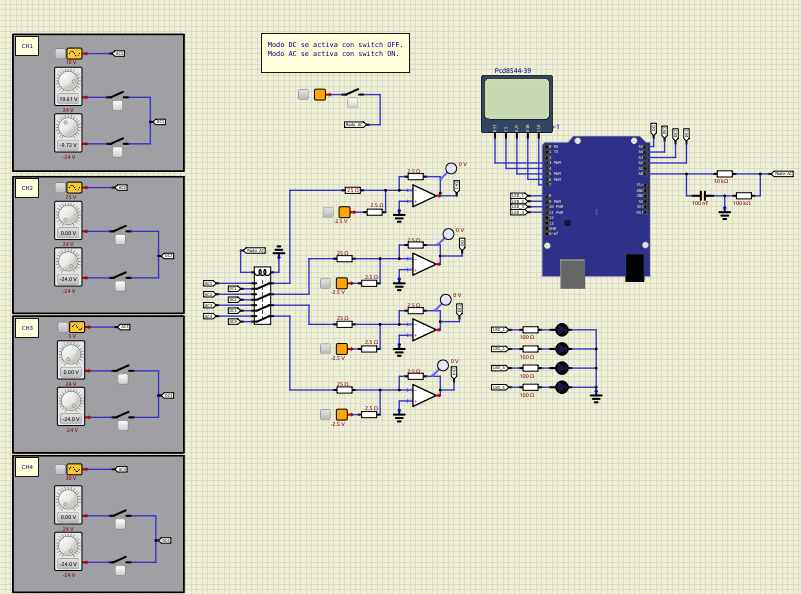
\includegraphics[width=.8\linewidth]{Imagenes/3.png}
 \caption{Circuito del voltímetro}
 \label{fig3}
\end{figure}

\newpage